
\section{Ejercicio 1}

Se consideran tres redes de interacci\'on prote\'inas de levadura: Red de 
copertenencia a complejos proteicos (AP-MS); Red de interacciones binarias 
(Y2H); y una red obtenida de la literatura (LIT), todas obtenidas del 
\textit{Yeast Interactome Database}, y mostradas en la figura \ref{fig:ej1_grafos}.

\begin{figure}[!ht]
    \centering
    \begin{subfigure}[b]{0.40\columnwidth}
        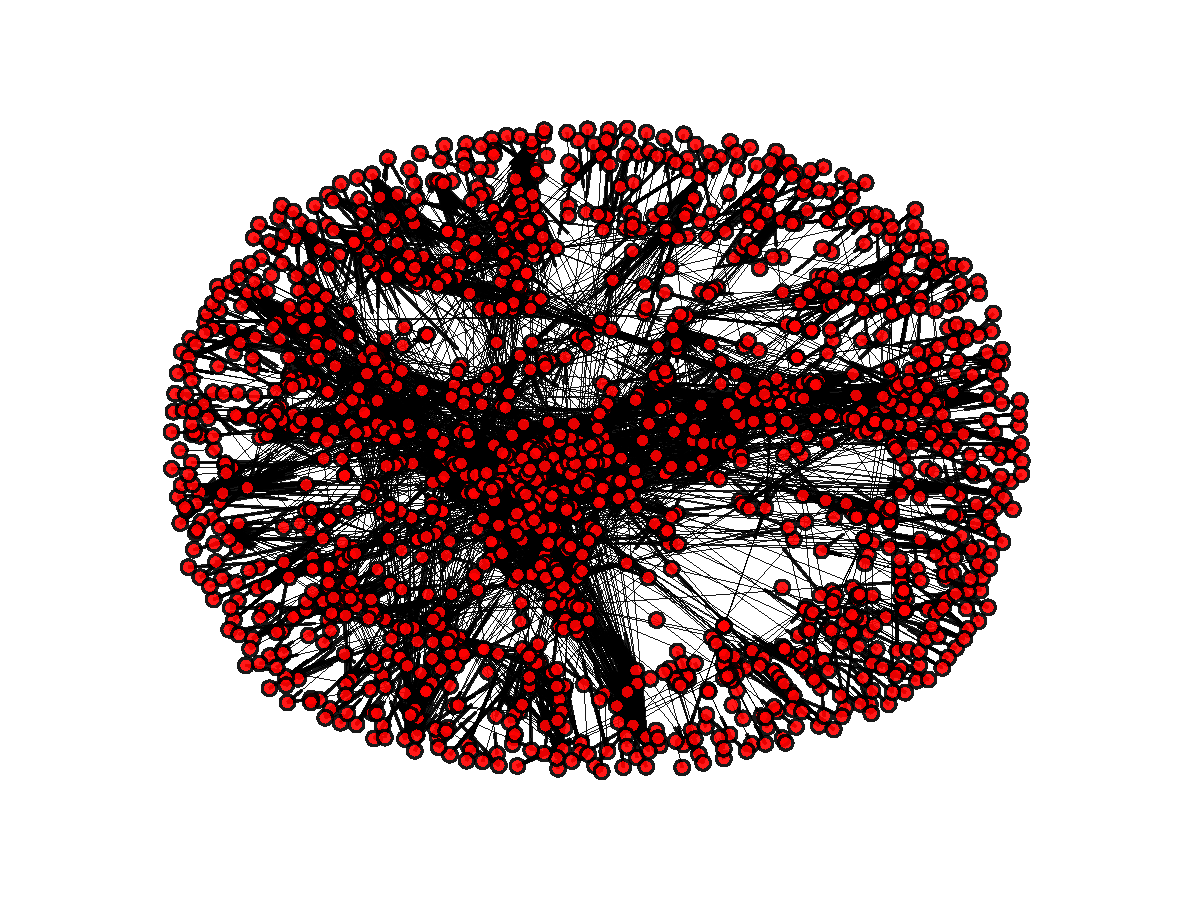
\includegraphics[width=\textwidth]{./schemes/yeast_AP-MS.pdf}
        \caption{\label{fig:ap_ms} AP-MS}
    \end{subfigure}
    \begin{subfigure}[b]{0.40\columnwidth}
        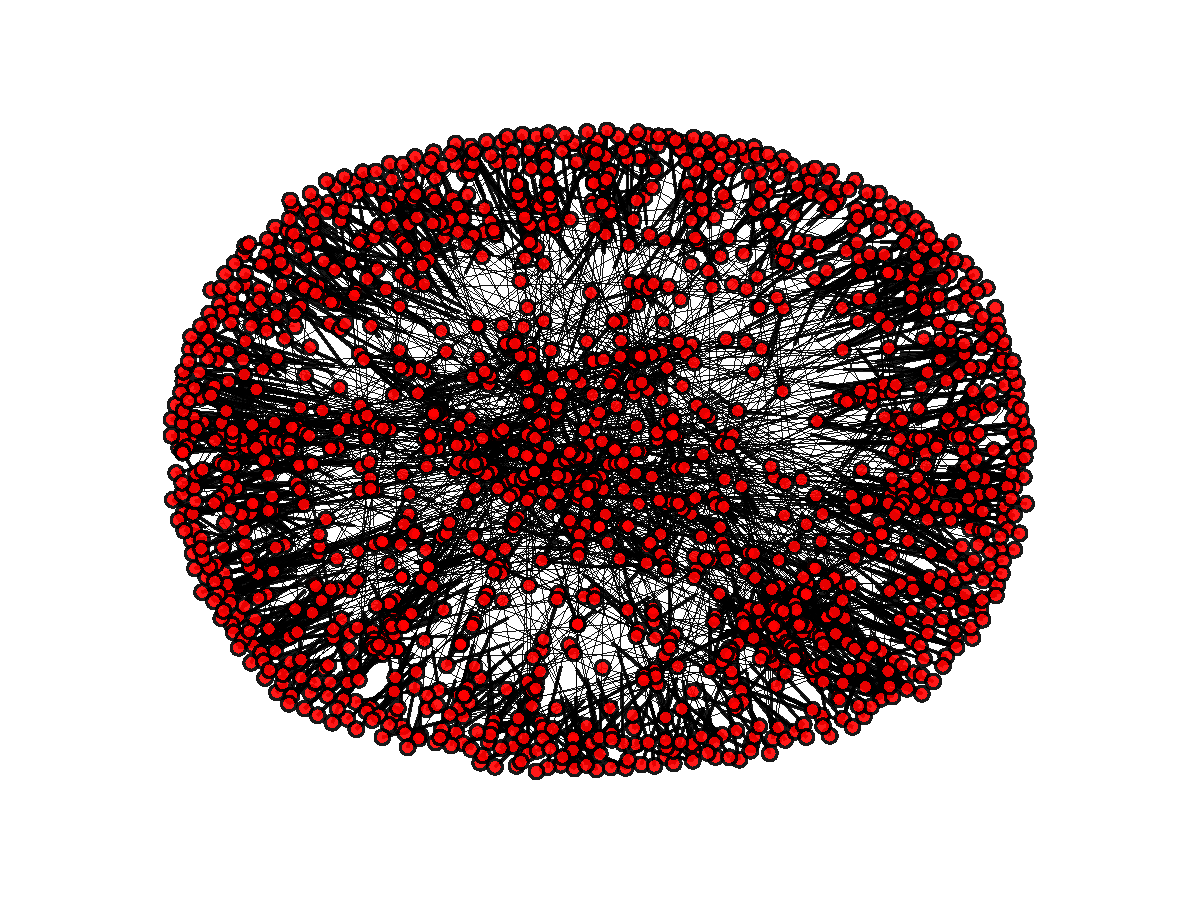
\includegraphics[width=\textwidth]{./schemes/yeast_LIT.pdf}
        \caption{\label{fig:LIT}LIT}
    \end{subfigure}
    \\
    \begin{subfigure}[b]{0.40\columnwidth}
        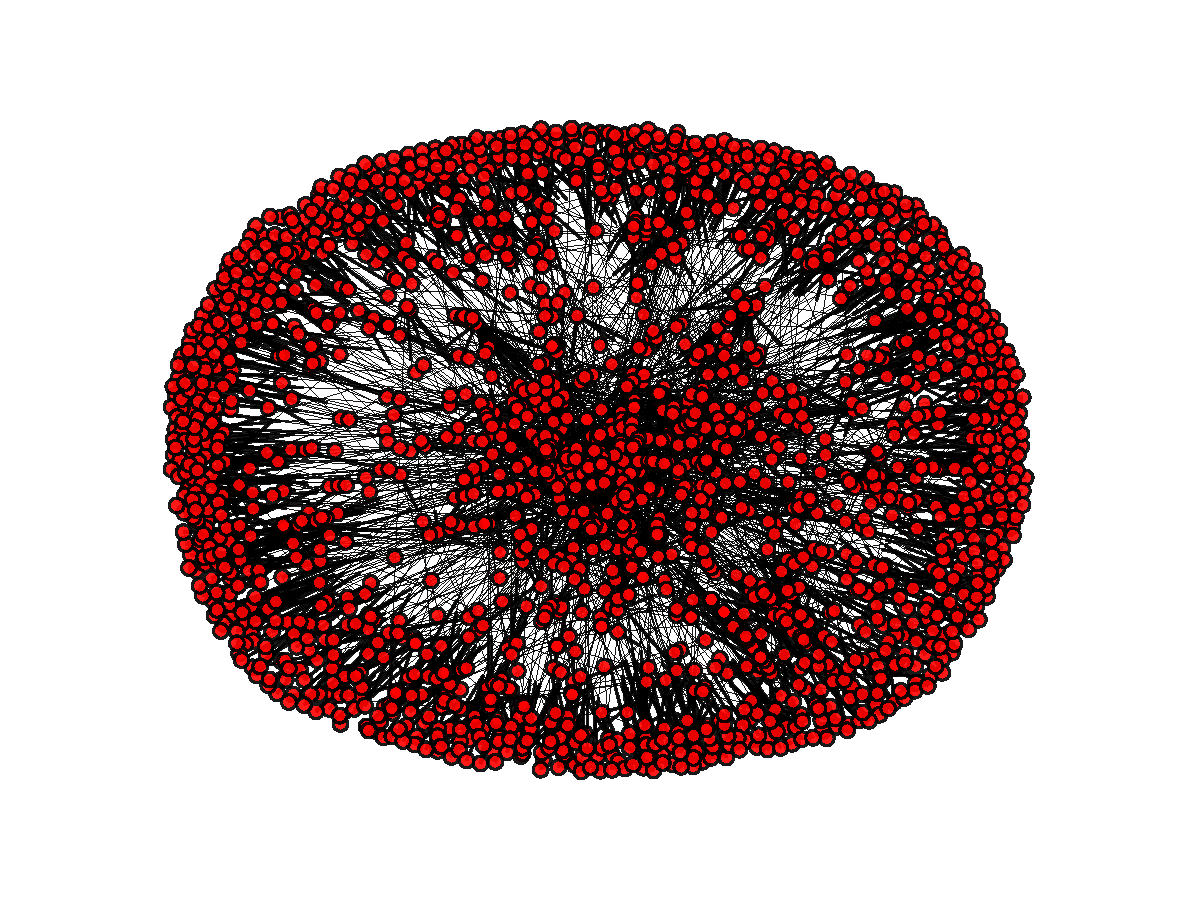
\includegraphics[width=\textwidth]{./schemes/yeast_Y2H.pdf}
        \caption{\label{fig:y2h} Y2H}
    \end{subfigure}
    \caption{\label{fig:ej1_grafos} Esquematizaci\'on de los grafos de cada 
    red estudiada. Se utiliz\'o un \textit{layout} estilo Frunchterman-Reigold 
    para la representaci\'on.}
\end{figure}

Graficamente se puede observar que la red Y2H tiene un nucleo bien definido
y un gran n\'umero de nodos conectados a \'el, esto significa que es posible
diferenciar dos grupos proteicos: Mediadoras (interaccionan con un gran
n\'umero de prote\'inas) y Mediadas (realizan alg\'un tipo de funci\'on con
ayuda de las mediadoras). El grupo de las Mediadoras (Nucleo) es probable 
que est\'e formado exlusivamente por enzimas.

Por otro lado en grafo AP-MS se pueden observar peque\~nos nucleos/clusters
muy conectados entre si y menos conectados con el resto. Estos nucleos dispersos
por la red son los complejos proteicos que busca carecterizar la red. 

\textbf{Que decir de la red LIT ??}\\


Una caracterizacion global y cuantitativa de las redes se muestra en la 
Tabla~\ref{tab:obs}. En ella se muestran diferentes observables globales
\textbf{Son realmente dirigidas ? analisis simple pero se debe tener claro
si se est\'a analizando lo correcto\ldots}
\begin{table}[!ht]
    \centering
    {\scriptsize
    \begin{tabularx}{1\columnwidth}{XlX|XcXcXcX}
        \hline\hline
        &Observables        &&& AP-MS && LIT && Y2H &\\ 
        \hline
        &Red dirigida       &&& Si && Si && Si &\\
        &Tiene loops        &&& No && Si && Si &\\
        &N$^o$ nodos $N$    &&& 1622 && 1536 && 2018 &\\
        &N$^o$ enlaces $L$  &&& 9070 && 2925 && 2930 &\\
        &Densidad           &&& 0.0034 && 0.0014 && 0.0007 &\\
        &Diametro           &&& 10 && 8 && 11 &\\
        \hline
        &Grado in $k_{in}$&&&\\
  %      \hline
        &\quad medio  $\mean{k_{in}}$     &&& 5.59 && 1.90 && 1.45 &\\
        &\quad maximo $\max(\{k_{in}\})$  &&& 111  && 23   && 66 &\\ 
        &\quad minimo $\min(\{k_{in}\})$  &&& 0    && 0    && 0 &\\ 
        \hline
        &Grado in $k_{out}$&&&\\
 %       \hline
        &\quad medio  $\mean{k_{out}}$     &&& 5.59 && 1.90 && 1.45 &\\
        &\quad maximo $\max(\{k_{out}\})$  &&& 85   && 35   && 38   &\\ 
        &\quad minimo $\min(\{k_{out}\})$  &&& 0    && 0    && 0    &\\ 
        \hline
        &Coeficiente de Clusterizaci\'on&&&\\
%        \hline
        &\quad medio/local $\mean{C}$               &&& 0.0741 && 0.4556 && 0.0970 & \\
        &\quad triangular/global $C_\bigtriangleup$ &&& 0.6185 && 0.3461 && 0.0236 & \\
        \hline\hline
    \end{tabularx}
    }
    \caption{\label{tab:obs}Observables para las tres redes de interacci\'on prote\'ica de levadura.}
\end{table}
        
    
\textbf{Diagrama de venn ???}
